\documentclass[pdf]{beamer}
\mode<presentation>{}
\usetheme{Warsaw}
\title{Prototype and Clustering Methods}
\subtitle{Breast Cancer Wisconsin Diagnostic Data Set}
\author{S.~Yang \and J.~Ensley \and M.~Mottahedi}
\subject{Data Mining}

\begin{document}

  \frame{\titlepage}

  \begin{frame}
    \frametitle{Data Set}
    \framesubtitle{Breast Cancer Wisconsin Diagnostic}
  \end{frame}

  \begin{frame}
    \frametitle{K-means}
    K-means
  \end{frame}

  \begin{frame}
    \frametitle{K-nearest neighbor}
    k-nearest neighbor
  \end{frame}


  \begin{frame}
    \frametitle{K-center}
    \framesubtitle{Unsupervised Clustering}
    Our goal is to find k circles that collectively enclose all the input points, such that the largest circle is as large as possible.
    Dividing the data into $2-6$ clusters:
    \begin{figure}
    \centering
    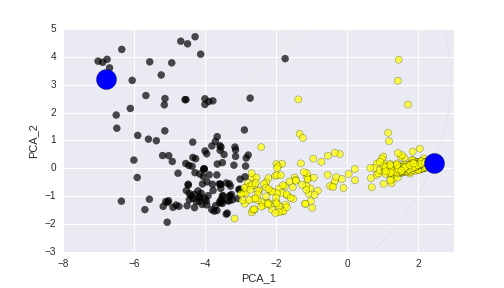
\includegraphics[width=0.5\textwidth]{m1.png}
    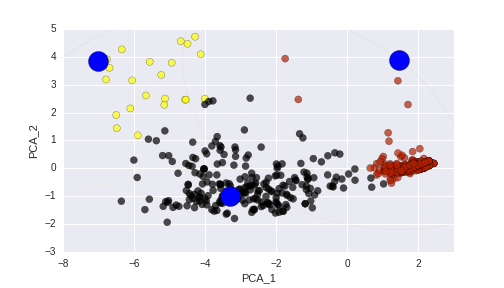
\includegraphics[width=0.5\textwidth]{m2.png}
    \caption{K-center unsupervised clustering results}
    \end{figure}


    \end{frame}

  \begin{frame}
    \frametitle{K-center}
    \framesubtitle{Unsupervised Clustering}

    \begin{figure}
    \centering
    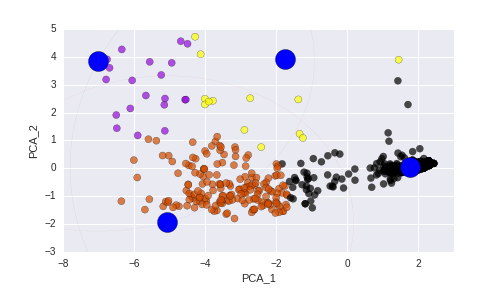
\includegraphics[width=0.5\textwidth]{m3.png}
    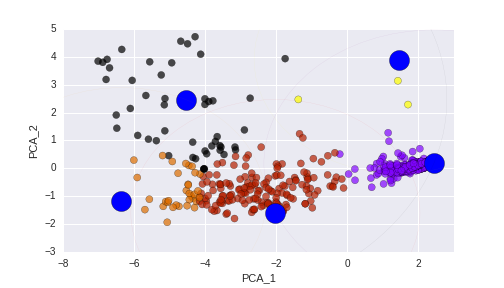
\includegraphics[width=0.5\textwidth]{m4.png}
    \end{figure}

    \begin{figure}
    \centering
    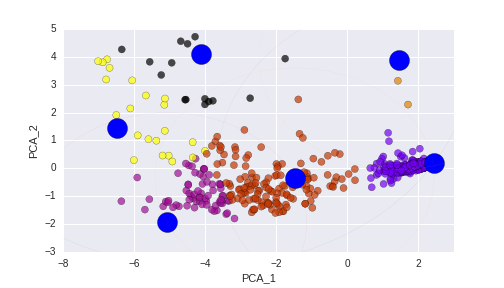
\includegraphics[width=0.5\textwidth]{m5.png}
    \caption{K-center unsupervised clustering results}
    \end{figure}

    \end{frame}


\end{document}